\documentclass[14pt]{extarticle}

\usepackage[english]{babel}
\usepackage[utf8]{inputenc}
\usepackage{graphicx,eso-pic}
\usepackage{tgschola}
\usepackage{listings}
\usepackage{pdfpages}
\usepackage[nodayofweek]{datetime}
\usepackage[bottom=2.25cm,top=3.75cm,left=1.5cm,right=1.5cm]{geometry}
\usepackage{xcolor}

\fontfamily{qcs}
\pagenumbering{gobble}

\lstdefinestyle{mystyle}{
    basicstyle=\small,       
    breaklines=true,                                 
    keepspaces=false,                                    
    numbersep=3pt,                  
    showspaces=false,                
    showstringspaces=false,
    showtabs=false,                  
    tabsize=1
}

\lstset{style=mystyle}

% Add header and footer images
\AddToShipoutPictureBG{%
  \AtPageUpperLeft{%
    \raisebox{-\height}{%
    
\includegraphics[width=\paperwidth]{private/header.jpeg}}
  }
  \AtPageLowerLeft{%
    \makebox{%
    
\includegraphics[width=\paperwidth]{private/footer.jpeg}}
  }
}

% Set title
\title{%
    \textbf{
    \vspace{-3em} \\ 
    \Large Experiment Number 4\\
    \vspace{-4em}
    }
}

% Remove author and Date
\author{}
\date{}

\begin{document}

\maketitle % Add title of doc

% Add the name and details
\section*{}
    \begin{tabular}{ llp{2cm}ll } 
        Name :: & Rishabh Anand & & UID :: & 19BCS4525  \\ 
        Branch :: & CSE - IoT & & Sec/Grp :: & 1/A \\ 
        Semester :: & 5\textsuperscript{th} & & Date :: & \shortdate{\today} \\
        Subject :: & Adv Programming Lab & & CODE :: & CSP-347  \\ 
        % Subject :: & Embedded System Lab & & CODE :: & CSD-333  \\ 
        % Subject :: & DIOT Lab & & CODE :: & CSD-337  \\ 
        % Subject :: & WSN Lab & & CODE :: & CSD-331  \\ 
    \end{tabular}
    
\vspace{1em}

\section*{\normalsize 1. Aim :}

Write a C++ program to read the a emp.dat file. Create new files such as Adm.dat, Sal.dat, Pro.dat, IT.dat respectively to store the employee details according to their department.

\section*{\normalsize 2. Task :}

\begin{enumerate}
  \item Write a C++ program to read the a emp.dat file. 
  \item Create new files such as Adm.dat, Sal.dat, Pro.dat, IT.dat respectively to store the employee details according to their department.
\end{enumerate}

% \section*{\normalsize 3. Theory :}

% \begin{enumerate}
%   \item 
% \end{enumerate}

\section*{\normalsize 3. Algorithm :}

\begin{enumerate}
  \item Read emp.dat file for current entries
  \item Take a number of entries
  \item Enter them in respective files.
  \item Save files.
  \item Exit
\end{enumerate}


% Auto add code and output
\newpage
\section*{\normalsize 4. Source Code :}

\lstinputlisting{temp/code.cpp} 

\newpage
\section*{\normalsize 5. Observations :}

\begin{center}
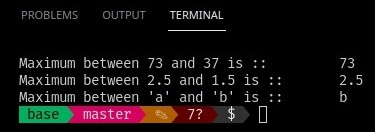
\includegraphics[scale=1.15]{temp/output.jpeg}
\end{center}

\section*{\normalsize Learning Outcomes :}
  
  \begin{itemize}
    \item File I/O
    \item ofstream
    \item ifstream
    \item fstream
  \end{itemize}

\section*{}

\begin{center}

\begin{tabular}{ |p{2.5cm}|p{4cm}|p{5cm}|p{5cm}|} 
 \hline
 S. No. & Parameters & Marks Obtained & Maximum Marks \\
 \hline
 1.&&&\\
 \hline
 2.&&&\\
 \hline
 3.&&&\\
 \hline
 &&&\\
 &&&\\
 \hline
\end{tabular}
\end{center}

\end{document}
